\chapter{Własne propozycje rozwiązań}
    \section{Pozyskanie i agregowanie danych} \label{data_aggregation}
    \noindent Pierwszym zadaniem, przed wykonaniem jakichkolwiek innych prac, było zebranie danych o meczach sportowych, które mogłyby być dalej używane do zadania uczenia maszynowego. W tym celu musiała zostać wykonana analiza odnalezionych wcześniej repozytoriów danych i ich odpowiednia transformacja, aby umieścić je we wspólnej bazie danych. W pracy zrezygnowano z płatnych źródeł takich jak wcześniej wspomniane \textit{Wyscout} czy \textit{StatsBomb}. Zdecydowano się wybrać darmowe repozytoria, które posiadały dobre opinie w literaturze lub w blogach internetowych i można było im zaufać. Każdy ze zbiorów posiadał pewne interesujące informacje, które uzupełniały się wzajemnie, co mogło pozwolić na uzyskanie spójnego zestawu ciekawych danych.
    
        \subsection{Europejska baza danych piłkarskich}
        \noindent Najważniejsze ze znalezionych repozytoriów stanowiła Europejska baza danych piłkarskich (\english{European Soccer Database})\footnote{\url{https://www.kaggle.com/hugomathien/soccer}}. Pochodzi ona z popularnej strony internetowej \url{www.Kaggle.com}, na której można znaleźć wiele zestawów danych powszechnie używanych do analizy przez społeczność analityków lub specjalistów uczenia maszynowego, którzy korzystają ze wspomnianego portalu. 
        
        Jest to utworzona w technologii SQLite baza danych zawierająca informacje na temat meczów ligowych odbywających się w Europie. Można tam znaleźć takie ligi jak niemiecka Bundesliga, polska Ekstraklasa oraz właśnie interesująca nas angielska Premier League. Zbiór pochodzi z roku 2016 i posiada mecze z sezonów od 2008 do 2016 roku. 
        Dane zebrane przez użytkownika Hugo Mathien, pochodzą z trzech wspomnianych przez niego źródeł.
        \begin{itemize}
            \item \url{http://football-data.mx-api.enetscores.com/} - według twórcy z tej strony pochodzą wyniki rozgrywek wraz ze szczegółowym opisem drużyn w tych właśnie meczach. Bezpośrednio strona juz jest niestety niedostępna, lecz można wejść na \url{https://www.enetscores.com/} i zauważyć, że zawierała ona wyniki na żywo dla różnych rozgrywek sportowych, wliczając w to piłkę nożną
            \item \url{http://www.football-data.co.uk/} - witryna z informacjami dotyczącymi kursów bukmacherskich dla lig piłkarskich,  w tym angielskiej. Więcej o tej stronie znaleźć można w rozdziale \ref{subsec:football-data}.
            \item \url{http://sofifa.com/} - portal zbierający dane z popularnej gry komputerowej FIFA. Europejska baza danych piłkarskich jest uzupełniona danymi o statystykach piłkarzy oraz drużyn pochodzącymi z corocznych edycji wspomnianego tytułu
        \end{itemize}
        Baza posiadała już określone relacje między encjami, które zostały zachowane w docelowej bazie danych utworzonej w systemie, w celu zachowania spójności udostępnionych danych. 
        
        Zbiór należało przenieść z technologii SQLite do Microsoft SQL Server. W tym celu wykorzystane zostało narzędzie do przeglądania baz danych typu SQLite, za pomocą którego zostały wyeksportowane poszczególne tabele do postaci skryptów języka SQL. Korzystając z tych skryptów można było zasilić bazę danych utworzoną w technologii Microsoft SQL Server uruchamiając je w odpowiedniej kolejności. Kolejnym krokiem było odfiltrowanie nieinteresujących danych w celu otrzymania bazy, która zawierała dane tylko o meczach ligi angielskiej. Z tego powodu odpowiednie zapytania posłużyły do usunięcia zbędnych danych i zachowania tylko tych, które posiadały wartość dla systemu, zgodnie z założeniami.
        
        \subsection{Elo Rating klubów piłkarskich}
        \noindent Parametr nazywany Elo rating, który był często wykorzystywany w badanych algorytmach uczenia maszynowego \cite{EloRating-1}, jest dostępny z strony internetowej \url{www.clubelo.com}. Można tam znaleźć dane nawet od roku 1939. Ranking utworzony na wspomnianym portalu powstał jedynie na podstawie meczów piłki nożnej i jest aktualizowany na bieżąco, obliczany przy pomocy algorytmu, który szczegółowo opisany jest na stronie, z której zostały pozyskane niezbędne dane\footnote{\url{http://clubelo.com/System}}.
        
        Pobieranie danych możliwe było z użyciem wystawionego web API\footnote{\url{http://clubelo.com/API}}, które umożliwiało pobranie pliku CSV, zawierającego historyczne informacje dla podanej drużyny.
        
        \subsection{Historyczne dane zakładów piłkarskich} \label{subsec:football-data}
         \noindent Wspomniane wcześniej dane dotyczące zakładów bukmacherskich meczów piłkarskich okazały się również dobrym źródłem danych, które zawierały informacje umożliwiające weryfikację zawartości i ewentualnie uzupełnienie tabeli, posiadającej dane o meczach. 
         
         \noindent Portal \url{http://www.football-data.co.uk/} udostępnia zestaw plików CSV dla poszczególnych lat wybranych meczów ligowych, w tym Premier League. Poszczególne pola zawarte w plikach opisane są na wspomnianej stronie internetowej\footnote{\url{https://www.football-data.co.uk/englandm.php}} i przy pomocy tych notatek pliki te zostały ,,rozszyfrowane'' i użyte w procesie uzupełniania tabel o brakujące dane. Informacje takie jak liczba strzałów, celnych strzałów, żółtych i czerwonych kartek, itd. można było znaleźć w tych plikach. Oprócz tego były tam wartości kursów zakładów bukmacherskich dla kilkunastu firm zajmujących się prowadzeniem takich gier hazardowych. Jak wcześniej, wg niektórych badaczy, wspomniane kursy zakładów to bardzo dobra cecha dla algorytmów predykcyjnych \cite{EloRating-1}, więc pobranie ich było także wybrane dla zapewnienia potencjalnie lepszej jakości systemu.
        
        \subsection{Metody agregacji}
        \noindent Ze względu na to, że dane pochodziły z różnych źródeł, trzeba było je zebrać i połączyć w odpowiedni sposób w celu otrzymania jednego spójnego zbioru, za pomocą którego można wyciągnąć informacje dla konkretnych rozgrywek. 
        
        Pierwszym krokiem było przeniesienie europejskiej bazy danych piłkarskich z SQLite do Microsoft SQL Server i odfiltrowanie odpowiednio nieinteresujących danych (np. mecze i zawodnicy pochodzący z innej ligi niż Premier League). Filtrowanie polegało na wyodrębnieniu wszystkich meczów z ligi angielskiej, po czym nastąpiło przepytanie bazy w poszukiwaniu wszystkich zawodników i drużyn biorących udział w tych rozgrywkach. Kolejno usunięte zostały wszystkie inne krotki drużyn i zawodników oraz odpowiadających im atrybutów. Tak samo mecze spoza ligi angielskiej zostały usunięte z bazy. Po wykonaniu wszystkich operacji, powstała kopia zapasowa bazy, która znajduje się na repozytorium projektu \cite{repo}, w folderze \textbackslash DataProjects\textbackslash MatchPredictDataImporter w pliku o nazwie \textit{Kaggle\_filtered.bacpac}, a przygotowana instancja została udostępniona na portalu Azure Cloud.
        
        Poza bazą danych zostały jeszcze dwa zbiory danych, które miały posłużyć do uzupełnienia utworzonego zestawu. W tym celu powstała solucja napisana w języku C\# przy użyciu framework'u  .Net Core w wersji 3.0 nazwana \textit{Match Predict Data Importer}. Działa ona w dwóch trybach:
        \begin{itemize}
            \item EloRatingImport - pobierane z web API wartości Elo rating dla przekazanych w pliku nazw drużyn i wstawienie ich do bazy danych do wcześniej przygotowanej tabeli EloRating. Łączenie z drużynami odbywa się po znalezieniu unikalnej drużyny z podanymi nazwami. Każda z drużyn posiada wiele wpisów w tabeli EloRating ze względu na to, że odnoszą się one do innych momentów w czasie. 
            \item KaggleFootballDataMerge - uzupełnienie danych w tabeli Match, przy pomocy pobranych ręcznie plików CSV z serwisu \url{http://www.football-data.co.uk/}. Niektóre pola wymagały wypełnienia, ponieważ nie zawierały one poprawnych danych dla statystyk poszczególnych drużyn podczas rozgrywki (np. liczba strzałów czy fauli). Połączenia między wartościami z pliku CSV, a wpisami w bazie były możliwe tylko wtedy, gdy mecz dla danej daty i pary drużyn występował w obu źródłach. Potwierdziło to prawdziwość danych, ponieważ dwa różne źródła się ze sobą pokrywały.
        \end{itemize}
        
        Wszelkie operacje na bazie danych, czy to pobieranie danych, czy ładowane wykonywane są przy pomocy biblioteki \textit{Entity Framework Core}, która zdecydowanie ułatwia to zadanie. Dzięki niej korzystając z dyrektyw języka C\# można operować na tabelach jak na klasach zdefiniowanych w projekcie bez konieczności pisania zapytań w języku SQL.
        
        Głównym problemem z importem danych z różnych źródeł była różnica w sposobie nazewnictwa drużyn. Jedynym sposobem na zidentyfikowanie drużyny dla przykładowo podpięcia do niej wartości Elo rating była jej nazwa. Jednak zespoły w przygotowanej bazie miały pełne nazwy (np. Manchester United), a aby pobrać Elo rating trzeba było wpisać specyficzną nazwę (np. dla drużyny Manchester United było to ManUnited). Spowodowało to konieczność ręcznego sprawdzenia każdej z drużyn i wpisaniu odpowiedniego mapowania do pliku podawanego na wejściu aplikacji. Taka sytuacja występowała zarówna dla trybu EloRatingImport jak i KaggleFootballDataMerge, oba posiadały różne mapowania nazw.
        
        Solucja została przetestowana przy pomocy testów jednostkowych przy wykorzystaniu biblioteki \textit{NUnit}, w celu zagwarantowania poprawności działania operacji.
        
        ~
        
        Całe rozwiązanie definiujące aplikację konsolową można znaleźć w repozytorium projektu \cite{repo} w folderze \textbackslash DataProjects\textbackslash MatchPredictDataImporter.
        
        
    \section{Web API}
    \noindent
    Posiadając spójnie zintegrowane dane umieszczone w bazie danych gotowe do użycia, następnym zadaniem było utworzenie wygodnego sposobu ich pobrania. W tym celu powstała solucja o nazwie \textit{Match Predict Data Provider}. Jak wspomniano w rozdziale \ref{arch:webApi} jest to tzw. web API utworzone w technologii \textit{Azure Function}, które wystawia dwa punkty końcowe. 
    
    Pierwsze pomysły zakładały dużą ilość pobierania danych tzw. drobnymi żądaniami, czyli np. zapytanie o mecze w danym sezonie, lecz zostało zauważone, że aby uzyskać szczegóły zawodników należało wykonać osobne żądanie dla każdego z osobna. Szybko okazało się to nieefektywne przez co zostały zastosowane inne podejścia.
    
    Wnioskiem nasuwającym się z analizy krytycznej poprzedniego pomysłu było pobieranie dużej ilości danych przy jednym zapytaniu, tj. mecze w danym sezonie wraz z wszystkimi możliwymi szczegółami, czyli każdy zawodnik i drużyna obecna w meczu przy jednym żądaniu. Ze względu na złożone zapytania do bazy danych skończyło się to długim czasem oczekiwania na odpowiedź (ok. 20 minut per sezon). Jedyną optymalizacją było dodanie indeksów na kluczach obcych, po których były często wykonywane łączenia, jednak nie spowodowało to widocznej poprawy. 
    
    Do tego samego punktu końcowego została dodana historia dla rozgrywających mecz drużyn, czyli określona przez parametr liczba meczów wstecz dla obu zespołów. Diametralnie wydłużyło to czas trwania zapytania, co spowodowało konieczność przemyślenia sposobu pobierania danych, aby nie wykonywać zbyt wielu niepotrzebnych zapytań do bazy danych.
    
    W celu minimalizacji zapytań, mecze wraz z drużynami i ich atrybutami są pobierane jednorazowo dla danego sezonu, po czym są wykorzystywane ponownie w celu poszukiwań przeszłych meczów. Jeżeli wśród pobranych rozgrywek nie znajduje się wystarczająca liczba historycznych meczów, są one dodatkowo pobierane jednorazowo. Należy dodać że mecze historyczne nie zawierają szczegółów, tylko i wyłącznie posiadają dane dotyczące wyników i innych statystyk meczu.
    
    Na potrzeby budowania cech dodana została również historia bezpośrednich rozgrywek między drużynami w analizowanym meczu i w podobny sposób zostaje obliczona jednorazowo dla każdej pary drużyn i wykorzystywana ponownie bez wykonywania zapytań. Kolejną dodaną informacją do żądania jest liczba punktów w poprzednim sezonie (jeśli jest dostępna). Obliczenie tej wartości wymaga wykonania zapytania, aby pobrać mecze z poprzedniego sezonu dla badanej drużyny, więc w celu ich minimalizacji zachowujemy wartość punktów w poprzednim sezonie w słowniku, przez co można ją wykorzystać, gdy dana drużyna pojawi się ponownie w innych meczach pobieranego sezonu.
    
    Wszelkie zabiegi optymalizacyjne doprowadził do żądań dostępu trwających ok. 2 minut, co zostało uznane za akceptowalny czas oczekiwania.
    
    \begin{figure}[H] 
        \centering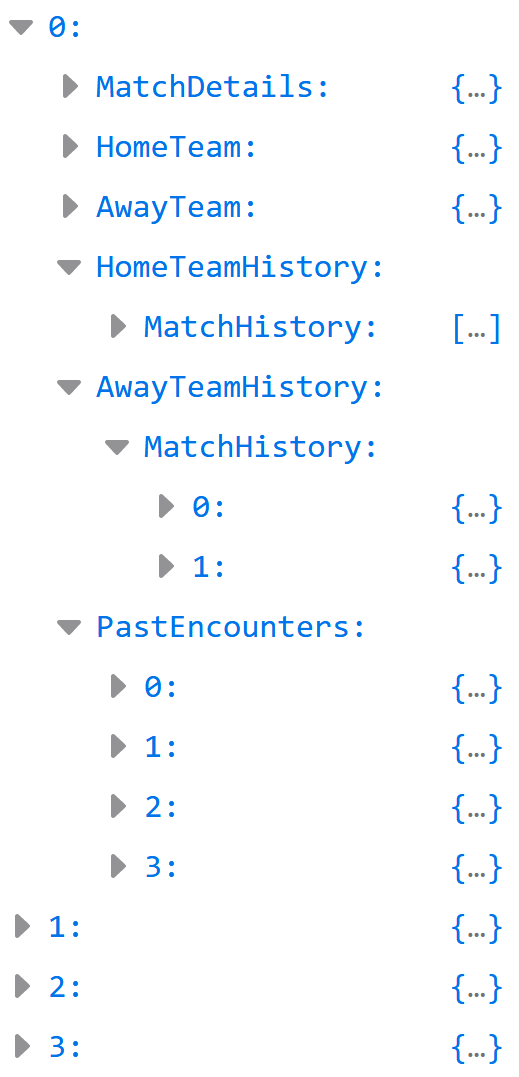
\includegraphics[width=4cm,height=8cm]{figures/example_response.png}
        \caption{Przykład odpowiedzi dla punktów końcowych web API}
        \label{fig:example_API_response}
    \end{figure}
    
    Na rysunku \ref{fig:example_API_response} można zauważyć sparsowany obiekt w formacie JSON, zwracany przez dostępne punkty końcowe. Jest to lista sformatowanych danych z tabel posiadająca następujące pola:
    \begin{itemize}
        \item MatchDetails - zrzut krotki z tabeli 'Match'

        \item HomeTeam - obiekt zawierający szczegóły drużyny gospodarzy znane przed zagranym meczem (krotka z tabeli 'Team'), w tym jej atrybuty (krotka z tabeli 'Team\_Attributes' dotycząca danej drużyny), liczba zagranych sezonów oraz liczba punktów w poprzednim sezonie
        \item AwayTeam - obiekt zawierający szczegóły drużyny gości, zawartość taka sama jak w przypadku drużyny gospodarzy
        \item HomeTeamHistory - klasa zawierająca listę meczów, zagranych przez drużynę gospodarzy w przeszłości
        \item AwayTeamHistory - klasa zawierająca listę meczów, zagranych przez drużynę gości w przeszłości
        \item PastEncounters - lista bezpośrednich starć drużyn grających w badanym meczu
    \end{itemize}
    
    Interfejsy budujące odpowiedzi na żądania zostały przetestowane testami jednostkowymi w celu upewnienia się, że każdy element poprawnie łączy ze sobą obiekty i zwraca oczekiwany wynik. Tak jak w przypadku projektu \textit{Match Predict Data Importer} wykorzystana zostałą biblioteka \textit{NUnit} języka C\#.
    
    Solucje zawierającą definicje web API można znaleźć w repozytorium projektu \cite{repo} w folderze \textbackslash DataProjects\textbackslash MatchPredictorDataProvider.
    
    \section{Wizualizacja charakterystyk danych}
    \noindent Przed przystąpieniem do właściwego przetwarzania danych oraz tworzenia na ich podstawie cech, uznano, że warto bliżej im się przyjrzeć w celu potwierdzenia ich prawidłowości i wyszukania potencjalnych błędów jak i braków. Ten podrozdział poświęcony jest wizualizacji charakterystyk danych, które są obecne w bazie. Wizualizacja została dokonana w języku Python w środowisku \emph{Jupyter Notebook}, a jej plik źródłowy znajduje się w repozytorium projektu~\cite{repo} w folderze \texttt{visualization/} pod nazwą \texttt{visualization.ipynb}
    
    Podczas wizualizacji pomijane są tabele, które są z jej punktu widzenia mało istotne - tabelę \emph{Team} (ponieważ zawiera ona tylko nazwy drużyn) i tabele \emph{Country} oraz \emph{League} (posiadają one tylko jeden wiersz - analizujemy rozgrywki z jednego kraju oraz jednej ligi). Podobnie z atrybutami - pomijane będą klucze podstawowe oraz klucze obce.
    
    ~
    
    Pierwszą tabelą wartą głębszej analizy jest tabela \emph{Team\_Attributes}. Zawiera ona pewne statystyki dla każdej z drużyn. Poniżej prezentuje się zestawienie kolumn tej tabeli wraz z ich typami i liczbą wartości niepustych:
    
    \begin{table}[H]
    \caption{Kolumny tabeli Team\_Attributes}
    \centering\footnotesize%
    \begin{tabular}{l c c}
    \toprule
        Nazwa & Liczba niepustych wartości & Typ \\
    \midrule
        date & 204 & datetime64 \\
        buildUpPlaySpeed & 204 & int64 \\
        buildUpPlaySpeedClass & 204 & int64 \\
        buildUpPlayDribbling & 68 & float64 \\
        buildUpPlayDribblingClass & 204 & string \\
        buildUpPlayPassing & 204 & float64 \\
        buildUpPlayPassingClass & 204 & string \\
        buildUpPlayPositioningClass & 204 & string \\
        chanceCreationPassing & 204 & int64 \\
        chanceCreationPassingClass & 204 & string \\
        chanceCreationCrossing & 204 & int64 \\ 
        chanceCreationCrossingClass & 204 & string \\        
        chanceCreationShooting & 204 & int64 \\  
        chanceCreationShootingClass & 204 & string \\
        chanceCreationPositioningClass & 204 & string \\
        defencePressure & 204 & int64 \\
        defencePressureClass & 204 & string \\
        defenceAggression & 204 & int64 \\  
        defenceAggressionClass & 204 & string \\
        defenceTeamWidth & 204 & int64 \\
        defenceTeamWidthClass & 204 & string \\
        defenceDefenderLineClass & 204 & string \\
    \bottomrule
    \end{tabular}
    \end{table}
    
    \noindent Wszystkich wierszy w tabeli jest 204, stąd na powyższym zestawieniu widać, że jedynym atrybutem, który nie ma uzupełnionych wartości dla wszystkich rekordów jest \emph{buildUpPlayDribbling}. Z uwagi na to, że brakujących wartości jest dosyć dużo (prawie 70\% wierszy w tabeli nie ma podanej wartości dla tego atrybutu), zdecydowano się go nie uwzględniać przy dalszym przetwarzaniu. Pomijane są również wszystkie kolumny typu \emph{string}, ponieważ są one tylko kategoriami (klasami) dla odpowiadających im wartości numerycznych.
    
    Przede wszystkim zdecydowano  przyjrzeć się histogramom wszystkich atrybutów numerycznych w celu weryfikacji poprawności ich rozrzutów wartości oraz skrajnych obserwacji na granicy zakresów.
    
    \begin{figure}[H] 
        \centering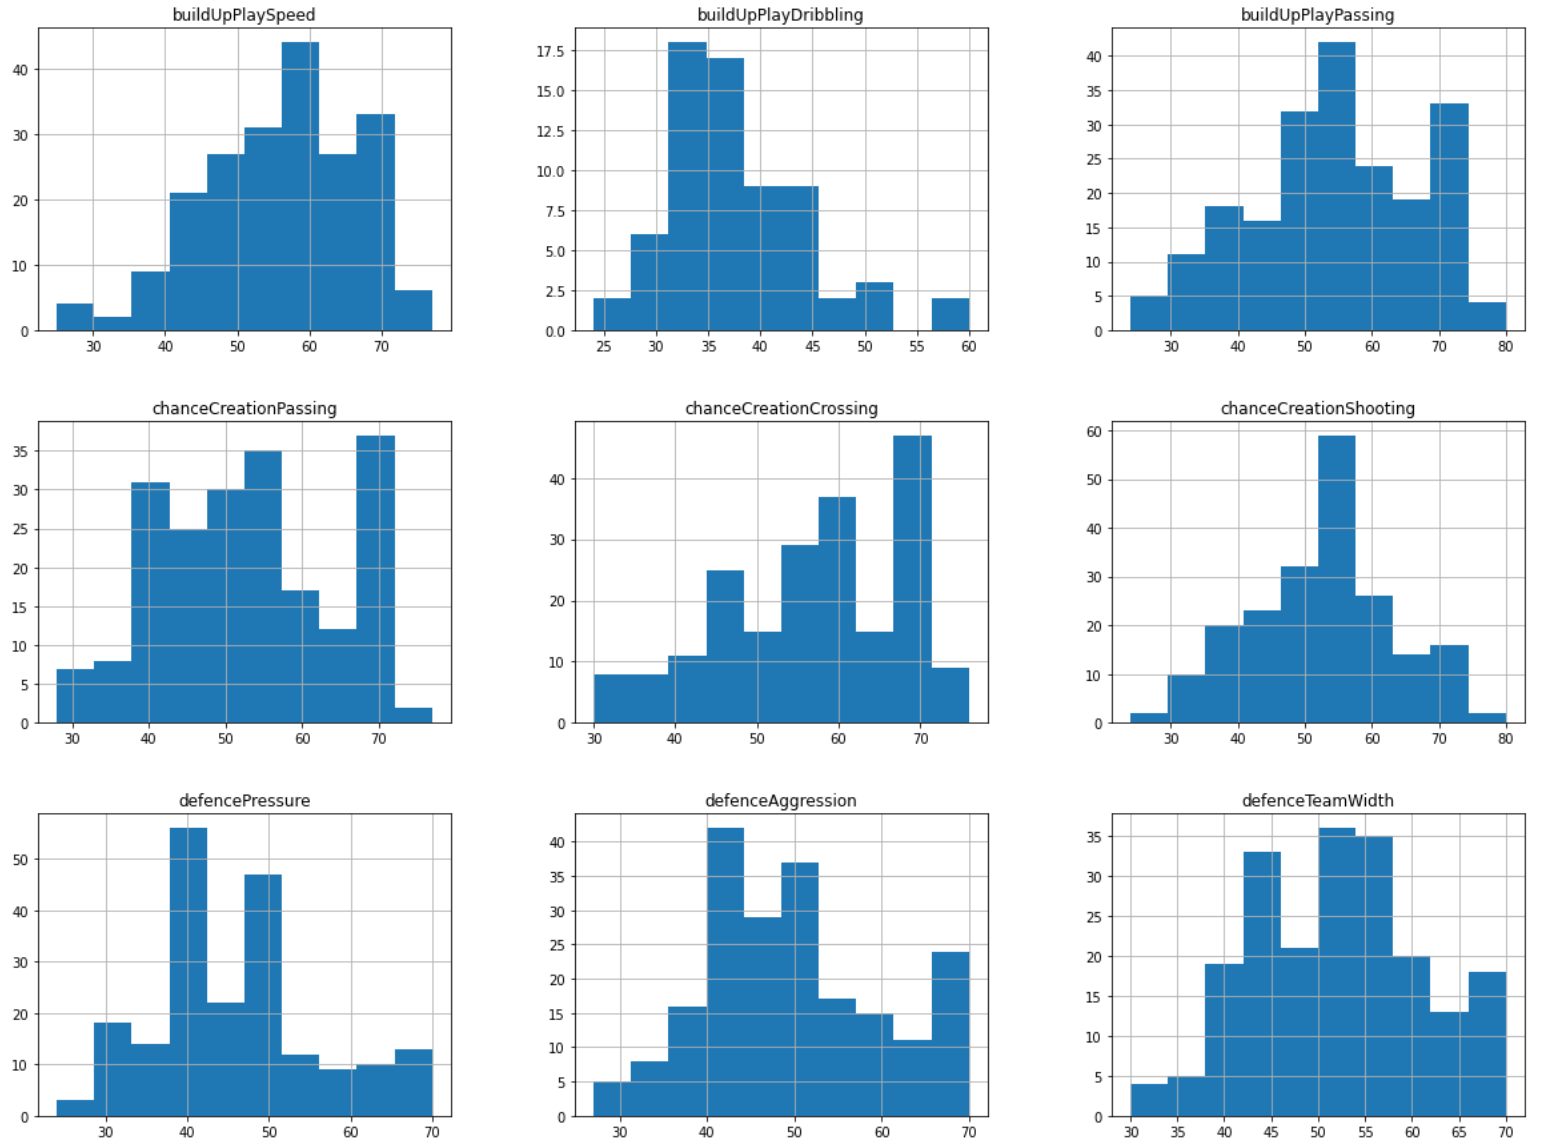
\includegraphics[width=\textwidth]{figures/team_attributes.png}
        \caption{Histogramy wartości numerycznych tabeli Team\_Attributes}
        \label{fig:team_attributes}
    \end{figure}
    
    \noindent Jak można zaobserwować na rysunku~\ref{fig:team_attributes}, wszystkie atrybuty mają odpowiednio wypełnione zakresy dziedzin - nie ma wartości odstających, ponadto wszystkie ich wartości są dodatnie. Uznano, że ich  dalsze przetwarzanie nie będzie konieczne.\\*
    
    \noindent Kolejną analizowaną tabelą jest tabela \emph{Player}. Posiada ona podstawowe informacje o wszystkich graczach.
    
    \begin{table}[H]
    \caption{Kolumny tabeli \emph{Player}}\label{tab:player}
    \centering\footnotesize%
    \begin{tabular}{l c c}
    \toprule
        Nazwa & Liczba niepustych wartości & Typ \\
    \midrule
        player\_name & 1397 & string \\
        birthday & 1397 & datetime64 \\
        height & 1397 & int64 \\
        weight & 1397 & int64 \\
    \bottomrule
    \end{tabular}
    \end{table}
    
    \noindent Wszystkich wierszy w tabeli Player jest 1397. Zgodnie z tablicą~\ref{tab:player}, tabela nie posiada wartości pustych. Z uwagi na trudność wizualizacji atrybutu \emph{birthday}, wprowadzony zostanie nowy, sztuczny atrybut wieku (\english{age}), który pozwoli zweryfikować jego poprawność. \\*
    
    \begin{figure}[H] 
        \centering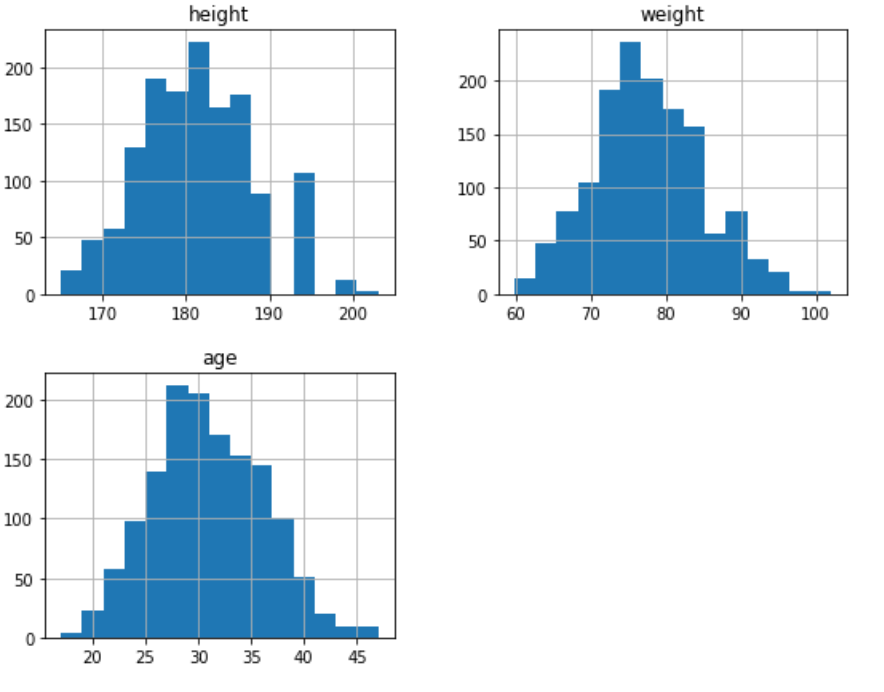
\includegraphics[width=\textwidth]{figures/player.png}
        \caption{Histogramy wartości dla atrybutów tabeli \emph{Player}}
        \label{fig:player}
    \end{figure}
    
    \noindent Spoglądając na rysunek~\ref{fig:player} zauważamy, że rozkłady wartości wszystkich atrybutów przypominają rozkłady normalne. Tutaj podobnie jak w przypadku poprzedniej tabeli, zakresy są poprawne. Warto zaznaczyć, że waga (\english{weight}) na potrzeby wizualizacji została przedstawiona w kilogramach, a wysokość (\english{height}) w centymetrach. Omówiony wcześniej sztuczny atrybut wieku pozwolił zweryfikować prawidłowość wartości dla kolumny \textit{birthday}. \\*
    
    \noindent Inną tabelą związaną z graczami jest tabela \emph{Player\_Attributes}. Zawiera ona pewne statystyki odnośnie każdego z graczy dotyczące jego umiejętności. Przyglądając się schematowi naszej bazy danych na rysunku~\ref{database_schema}, można zaobserwować, że tabela ta posiada dużo różnych atrybutów numerycznych. Istotne jednak z punktu widzenia późniejszego tworzenia cech jest istnienie atrybutu zwanego \emph{overall\_rating}, który można na język polski przetłumaczyć jako ,,ogólna ocena''. Jest on pewną agregacją wszystkich pozostałych atrybutów dokonaną przez twórców gry FIFA. Dzięki niemu można pominąć pozostałe atrybuty i do dalszego przetwarzania uwzględnić wyłącznie ten.
    
    \begin{figure}[H] 
        \centering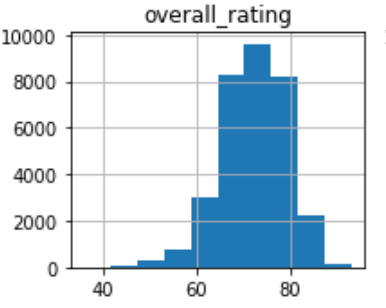
\includegraphics[width=5cm]{figures/overall_rating.png}
        \caption{Histogram wartości atrybutu \emph{overall\_rating}}
        \label{fig:overall_rating}
    \end{figure}
    
    \noindent Dodatkowym jego atutem, co można zauważyć na rysunku~\ref{fig:overall_rating}, jest w miarę regularny przebieg  zakresu jego wartości oraz fakt, że jest on zdefiniowany dla każdego gracza w bazie danych.
    
    Atrybuty kategoryczne, m.in \emph{preferred foot} (,,preferowana noga''), zostały pominięte ze względu na wątpliwy wpływ na predykcję wyniku meczu. \\*
    
    \noindent \emph{EloRating} jest tabelą, która zawiera wartości tzw. atrybutu \emph{Elo} aktualnego na dany dzień dla każdej z drużyn.
    
    \begin{table}[H]
    \caption{Kolumny tabeli EloRating}\label{tab:elo}
    \centering\footnotesize%
    \begin{tabular}{l c c}
    \toprule
        Nazwa & Liczba niepustych wartości & Typ \\
    \midrule
        team\_name & 31607 & string \\
        rank & 31607 & int64 \\
        Elo & 31607 & float64 \\
        start\_date & 31607 & datetime64 \\
        end\_date & 31607 & datetime64 \\
    \bottomrule
    \end{tabular}
    \end{table}
    
    \begin{table}[H]
    \caption{Przykładowe rekordy w tabeli EloRating}\label{tab:elo_example}
    \centering\footnotesize%
    \begin{tabular}{l c c c c}
    \toprule
        team\_name & rank & Elo & start\_date & end\_date \\
    \midrule
        Manchester United & 14 & 1843.027344 & 2014-08-17 & 2014-08-19\\
        Manchester United & 14 & 1842.388550 & 2014-08-20 & 2014-08-21\\
        Manchester United & 15 & 1840.082642 & 2014-08-22 & 2014-08-23\\
        Manchester United & 14 & 1840.082642 & 2014-08-24 & 2014-08-24\\
        Manchester United & 14 & 1836.078979 & 2014-08-25 & 2014-08-27\\
        Manchester United & 15 & 1837.623047 & 2014-08-28 & 2014-08-28\\
    \bottomrule
    \end{tabular}
    \end{table}
    
    \noindent Tablica~\ref{tab:elo} stanowi potwierdzenie uzupełnionych wartości atrybutów dla każdego rekordu w tabeli, a tablica~\ref{tab:elo_example} obrazuje, że dla każdej drużyny w naszej bazie może istnieć wiele rekordów. Każdy zawiera inną wartość atrybutu \emph{Elo} (wraz z miejscem zajmowanym w globalnym rankingu drużyn) aktualnym w danym przedziale czasowym. Atrybut ten ulega przeliczeniu po każdym rozegranym przez drużynę meczu.
    
    Tworząc wektory cech reprezentujące pojedynczy mecz, dla obu drużyn korzystamy z wartości tego atrybutu aktualnego na dzień meczu. Obrazuje on aktualną ,,formę'' drużyny w dniu rozgrywania meczu. \\*
    
    \noindent Najobszerniejszą tabelą w naszym systemie jest tabela \emph{Matches}. Każdy jej rekord reprezentuje jeden mecz pomiędzy dwoma drużynami wraz z jego charakterystykami, np. liczba strzałów drużyny gospodarzy, liczba żółtych kartek drużyny gości, kursy oferowane na remis itd.
    
    Z uwagi na sporą liczbę atrybutów w tej tabeli, warto ją podzielić na mniejsze części w celu łatwiejszej i czytelniejszej analizy. Pierwszą badanym zestawem są atrybuty związane z kursami od różnych zakładów bukmacherskich.
    
    \begin{table}[H]
    \caption{Podstawowe statystyki dla atrybutów związanych z kursami.}\label{tab:odds}
    \centering\footnotesize%
    \begin{tabular}{l c c c c c}
    \toprule
        Atrybut & \emph{count} & \emph{mean} & \emph{std} & \emph{min} & \emph{max} \\
    \midrule
        B365H & 3040 & 2.701964 & 1.689834 & 1.100000 & 15.000000\\
        BWH & 3039 & 2.603906 & 1.528913 & 1.100000 & 12.500000\\
        IWH & 3038 & 2.513644 & 1.368492 & 1.050000 & 10.000000\\
        LBH & 3039 & 2.611787 & 1.526034 & 1.080000 & 12.000000\\
        PSH & 1519 & 2.720369 & 1.575303 & 1.130000 & 10.800000\\
        WHH & 3040 & 2.663760 & 1.590124 & 1.100000 & 12.000000\\
        SJH & 2320 & 2.667828 & 1.698067 & 1.110000 & 15.000000\\
        VCH & 3040 & 2.712204 & 1.692001 & 1.090000 & 15.000000\\
        GBH & 1899 & 2.606840 & 1.586001 & 1.100000 & 12.000000\\
        BSH & 1900 & 2.625553 & 1.655792 & 1.100000 & 13.000000\\\\
        
        B365D & 3040 & 3.952720 & 0.998305 & 3.000000 & 11.000000\\
        BWD & 3039 & 3.803251 & 0.882597 & 2.900000 & 9.250000\\
        IWD & 3038 & 3.687903 & 0.735121 & 3.000000 & 10.000000\\
        LBD & 3039 & 3.815271 & 0.876612 & 2.880000 & 10.000000\\
        PSD & 1519 & 4.078183 & 1.046468 & 3.040000 & 11.030000\\
        WHD & 3040 & 3.669260 & 0.812509 & 2.800000 & 9.500000\\
        SJD & 2320 & 3.881039 & 0.926573 & 3.000000 & 9.000000\\
        VCD & 3040 & 3.955470 & 1.009081 & 2.500000 & 10.000000\\
        GBD & 1899 & 3.761980 & 0.842088 & 3.000000 & 8.500000\\
        BSD & 1900 & 0.837965 & 0.837965 & 3.000000 & 8.500000\\\\
        
        B365A & 3040 & 4.910437 & 3.909392 & 1.220000 & 29.000000\\
        BWA & 3039 & 4.495166 & 3.213833 & 1.220000 & 21.000000\\
        IWA & 3038 & 4.245671 & 2.919038 & 1.270000 & 25.000000\\
        LBA & 3039 & 4.563537 & 3.371435 & 1.220000 & 26.000000\\
        PSA & 1519 & 4.923970 & 3.840303 & 1.370000 & 28.500000\\
        WHA & 3040 & 4.699592 & 3.628486 & 1.220000 & 26.000000\\
        SJA & 2320 & 4.859233 & 3.826951 & 1.250000 & 29.000000\\
        VCA & 3040 & 4.956711 & 3.984335 & 1.220000 & 29.000000\\
        GBA & 1899 & 4.566435 & 3.301710 & 1.250000 & 21.000000\\
        BSA & 1900 & 3.786069 & 3.786069 & 1.220000 & 26.000000\\
    \bottomrule
    \end{tabular}
    \end{table}
    
    \noindent Tablica~\ref{tab:odds} zawiera pogrupowane kursy od różnych bukmacherów według zdarzeń. Ostatnia litera w nazwie atrybutu informuje o typie zdarzenia, na który jest oferowany ten kurs. Litera ,,H'' oznacza kurs oferowany na zwycięstwo drużyny gospodarzy, ,,D'' na remis, natomiast ,,A'' na zwycięstwo gości. Pozostałe litery tworzą skrót od nazwy danego bukmachera. Prezentowane statystyki to liczność (\english{count}) średnia (\english{mean}), odchylenie standardowe (\english{standard deviaton, std}), wartość minimalna oraz maksymalna.
    
    Jak można spostrzec analizując wartości średnie dla poszczególnych grup, na zwycięstwo gospodarzy oferowany jest średnio mniejszy kurs niż na pozostałe dwa zdarzenia. Pozwala to podejrzewać, że granie na swoim stadionie daje drużynie pewną przewagę. Potwierdza to fakt, że na zwycięstwo gości średnio ten kurs jest najwyższy.
    
    Warto również zwrócić uwagę na to, że w obrębie poszczególnych grup zdarzeń, średnie kursy proponowane przez bukmacherów są bardzo do siebie zbliżone. Oznacza to, że najprawdopodobniej ich modele matematyczne wyznaczają podobne prawdopodobieństwa dla danych zdarzeń. Dodatkowym istotnym faktem jest to, że dla każdej grupy zdarzeń istnieją przynajmniej dwa atrybuty, które są zdefiniowane dla każdego meczu (których liczność w naszej bazie danych wynosi 3400). Przykładowo, dla zdarzeń z grupy ,,zwycięstwo gospodarzy'' zawsze istnieje wartość dla atrybutu \emph{B365H} oraz \emph{WHH} (ich wartość \emph{count} wynosi 3040). Ten fakt, wraz z obserwacją o podobnych kursach w obrębie poszczególnych grup, umożliwiają poradzenie sobie z brakującymi wartościami niektórych atrybutów. Skoro wiadomo, że kursy na dane zdarzenie są podobne, wystarczy uwzględniać podczas późniejszego przetwarzania tylko te atrybuty, które mają wartość niepustą (mamy gwarancję obecności przynajmniej dwóch takich atrybutów dla każdego z trzech zdarzeń w meczu- zwycięstwa gospodarzy, remisu oraz zwycięstwa gości). \\*
    
    \noindent Kolejnym zestawem analizowanych atrybutów są te związane bezpośrednio z przebiegiem meczu. 
    
    \begin{table}[H]
    \caption{Wybrane atrybuty tabeli \emph{Matches}}\label{tab:matches}
    \centering\footnotesize%
    \begin{tabular}{l c c l}
    \toprule
        Nazwa & Liczba niepustych wartości & Typ & Wyjaśnienie \\
    \midrule
        HomeTeamShots & 3040 & int64 & liczba strzałów drużyny gospodarzy \\
        AwayTeamShots & 3040 & int64 & liczba strzałów drużyny gości \\
        HomeTeamShotsOnTarget & 3040 & int64 & liczba celnych strzałów drużyny gospodarzy \\
        AwayTeamShotsOnTarget & 3040 & int64 & liczba celnych strzałów drużyny gości \\
        HomeTeamCorners & 3040 & int64 & liczba rzutów rożnych drużyny gospodarzy \\
        AwayTeamCorners & 3040 & int64 & liczba rzutów rożnych drużyny gości \\
        HomeTeamFoulsCommitted & 3040 & int64 & liczba popełnionych fauli przez gospodarzy \\
        AwayTeamFoulsCommitted & 3040 & int64 & liczba popełnionych fauli przez gości \\
        HomeTeamYellowCards & 3040 & int64 & liczba żółtych kartek otrzymanych przez gospodarzy \\
        AwayTeamYellowCards & 3040 & int64 & liczba żółtych kartek otrzymanych przez gości \\
        AwayTeamRedCards & 3040 & int64 & liczba czerwonych kartek otrzymanych przez gości \\
        HomeTeamRedCards & 3040 & int64 & liczba żółtych kartek otrzymanych przez gospodarzy \\
    \bottomrule
    \end{tabular}
    \end{table}

     \begin{figure}[H] 
        \centering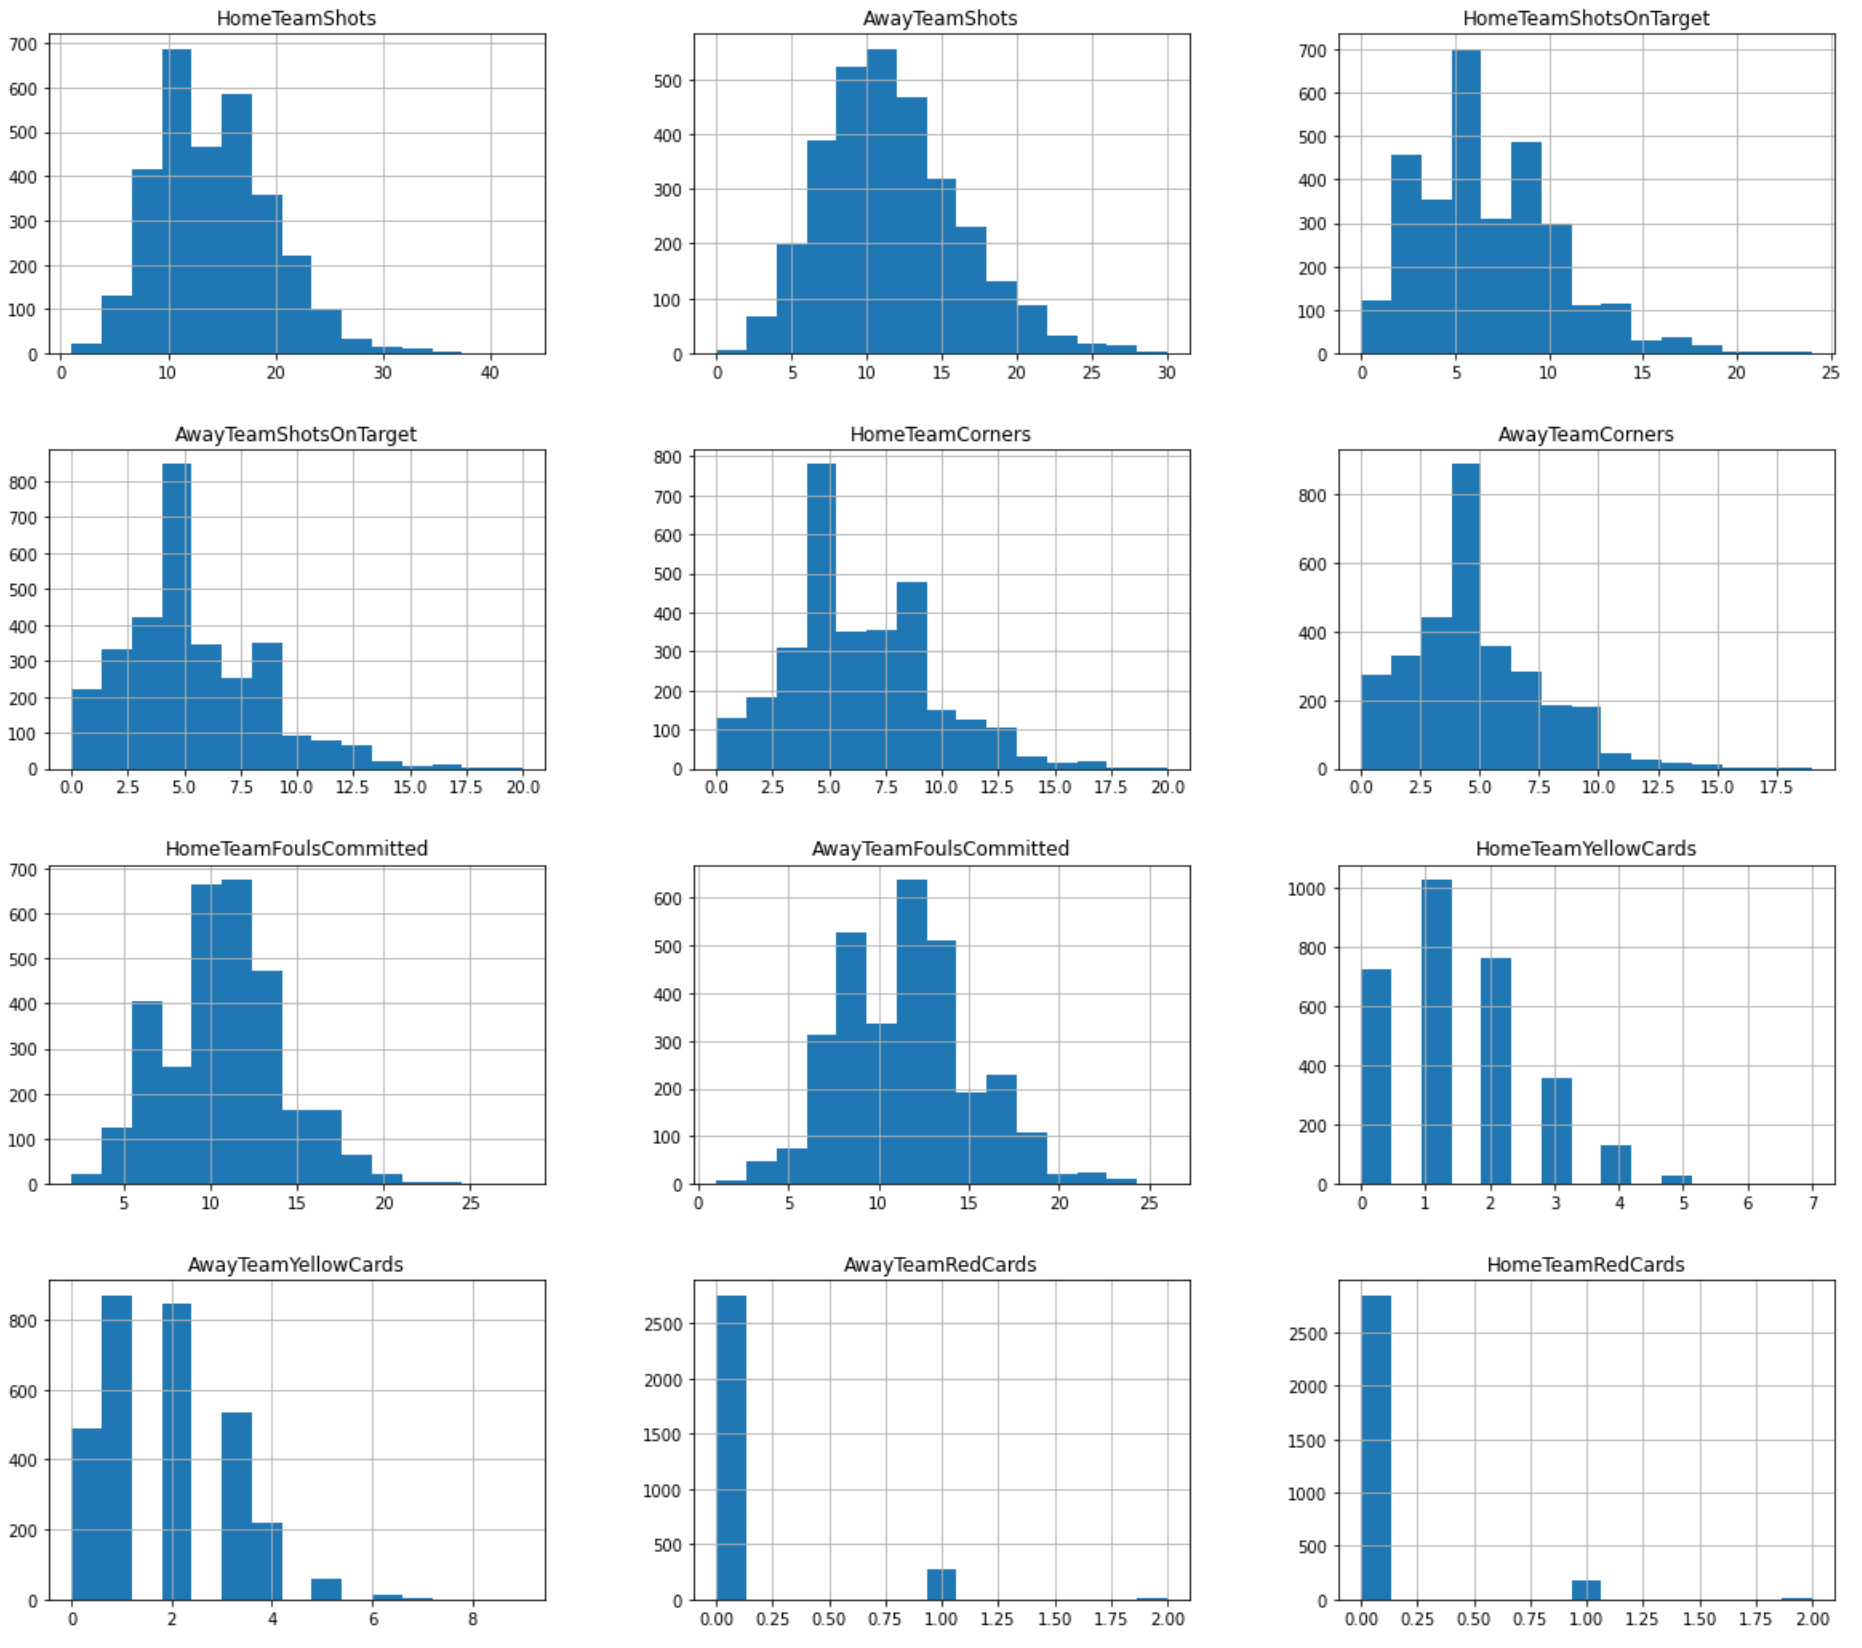
\includegraphics[width=\textwidth]{figures/matches.png}
        \caption{Histogramy wybranych atrybutów tabeli \emph{Matches}}
        \label{fig:matches}
    \end{figure}
    
    \noindent Tablica~\ref{tab:matches} utwierdza nas w przekonaniu, iż wszystkie atrybuty są uzupełnione i nie zawierają żadnych brakujących wartości.
    Na rysunku~\ref{fig:matches} przedstawiono ich histogramy. Potwierdzają one pełen rozkład zakresów wartości bez nietypowości, jak i pewne intuicyjne założenia, przykładowo - czerwone kartki są sporadycznym zdarzeniem i występują zdecydowanie rzadziej niż żółte kartki. 
    
    \section{Wstępne przetwarzanie}
    \noindent Na rysunku~\ref{fig:preprocessing_structure} przedstawiona została struktura modułu służącego do pobierania danych z serwera, ich wstępnego przetwarzania oraz tworzenia na ich podstawie cech. Moduł ten znajduje się w repozytorium projektu~\cite{repo} w folderze \texttt{Preprocessing/}.
    \begin{figure}[H] 
        \centering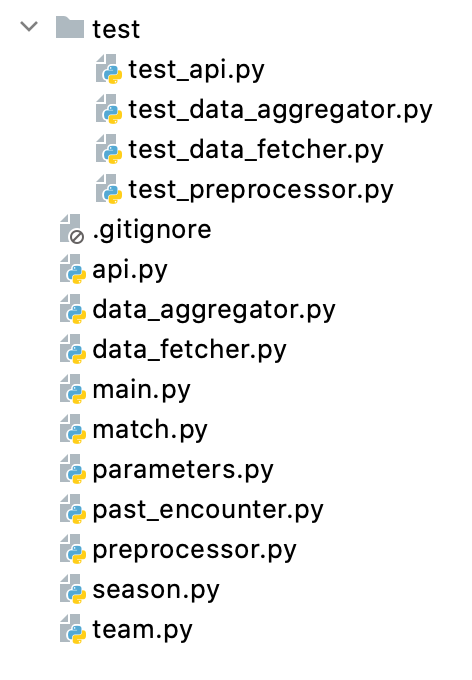
\includegraphics[width=6cm]{figures/preprocessing_structure.png}
        \caption{Struktura modułu do wstępnego przetwarzania}
        \label{fig:preprocessing_structure}
    \end{figure}
    
    Oprócz podfolderu \texttt{test/} (który zostanie szczegółowo omówiony w późniejszym podrozdziale) przechowującego wszystkie testy jednostkowe, znajdują się w nim też właściwe pliki odpowiedzialne za wspomniane funkcje modułu:
    
    \begin{itemize}
        \item \texttt{api.py} - plik zawierający funkcje pomocnicze do tworzenia odpowiedniego url'a, przy pomocy którego następuje wysłanie zapytanie do serwera,
        \item \texttt{data\_fetcher.py} - odpowiada za pobieranie danych z serwera przy użyciu \emph{web API},
        \item \texttt{data\_aggregator.py} - używa poprzedniego pliku w celu pobrania danych i służy do ich agregacji (np. danych dla kilku sezonów) w jeden zbiór danych; jest punktem wejściowym do biblioteki, który używa klient,
        \item \texttt{preprocessor.py} - przetwarza otrzymane dane i tworzy na ich podstawie wektory cech reprezentujące każdy mecz,
        \item \texttt{match.py}, \texttt{parameters.py}, \texttt{past\_encounters.py}, \texttt{season.py} oraz \texttt{team.py} - reprezentują modele danych używane w systemie i enkapsulują ich pewne właściwości (np. identyfikator dla sezonu lub drużyny, który jest potrzebny do wykonania zapytania do serwera),
        \item \texttt{main.py} - zawiera przykład użycia biblioteki.
    \end{itemize}
    
        \subsection{Pobieranie danych z serwera i ich agregacja}
        \noindent Moduł komunikuje się z serwerem przy pomocy udostępnionego przez niego interfejsu programistycznego. Komunikacja ta jest inicjowana przez klienta przy użyciu dwóch funkcji z pliku \texttt{data\_aggregator.py}:
        
        \begin{itemize}
            \item \texttt{get\_data\_for\_seasons()}
            \item \texttt{get\_data\_for\_team\_in\_seasons()}
        \end{itemize}
        
        Obie te funkcje przyjmują jako argument listę sezonów, dla których mają być pobrane dane oraz obiekt \emph{Parameters}, który pozwala sparametryzować zapytanie do serwera. Obiekt ten aktualnie posiada tylko jeden atrybut, który określa ile meczów z przeszłości dla danej drużyny brać pod uwagę przy pobieraniu danych.
        
        Dodatkowo, druga z funkcji pozwala na określenie drużyny, dla której mają być pobrane dane. Oto jak wygląda przykładowe wywołanie obu tych funkcji.
        
        \begin{lstlisting}[language=Python, label={lis:example_usage}, caption=Przykładowe wywołanie funkcji do pobrania danych]
        data_aggregator = DataAggregator()
        
        # pobierz dane dla sezonu 2011 i 2012
        data_aggregator.get_data_for_seasons([Season.y2011, Season.y2012], Parameters(no_last_matches=3))
        
        # pobierz dane dla Arsenalu z sezonu 2011 i 2012
        data_aggregator.get_data_for_team_in_seasons(Team.Arsenal, [Season.y2011, Season.y2012], Parameters(no_last_matches=3))
        \end{lstlisting}
        
        \noindent Zapytanie do serwera pozwala na pobranie danych jednorazowo dla konkretnego sezonu lub drużyny. Natomiast jak można zauważyć na listingu \ref{lis:example_usage}, klient ma możliwość wykonania zapytania dla kilku sezonów naraz. Tę możliwość udostępnia klasa \emph{DataAggregator}, która wewnętrznie wykonuje osobno zapytanie dla każdego sezonu i agreguje otrzymane dane w jeden zbiór, który zwracany jest klientowi.
        
        W celu pobrania danych, klasa \emph{DataAggregator} korzysta z klasy znajdujacęj się we wcześniej wspomnianym pliku \texttt{data\_fetcher.py} o nazwie \emph{DataFetcher}. Na listingu \ref{lis:data_fetcher} widać fragment tej klasy. Przy wykonywaniu zapytania, najpierw korzysta ona z funkcji pomocniczej do stworzenia odpowiedniego url'a, a później wykonuje faktyczne zapytanie i zwraca jego wynik. Warto również zwrócić uwagę na mechanizm z pamięcią podręczną. Po otrzymaniu odpowiedzi od serwera, jest ona zapisywana w pamięci pod odpowiednim kluczem. Przed wykonaniem zapytania do serwera, sprawdzane jest, czy nie zostało już wcześniej wykonane zapytanie z takimi samymi parametrami. Jeżeli tak, zwracany jest jego wynik.
        
        
        \begin{lstlisting}[language=Python, label={lis:data_fetcher}, caption=Fragment klasy \emph{DataFetcher}]
        class DataFetcher:

            def __init__(self):
                self.cache = {}

            def fetch_data_for_season(self, season, params):
                url = get_url_for_matches_in_season(season.value, params)
                if url in self.cache:
                    return self.cache[url]
                data = requests.get(url).text
                self.cache[url] = data
                return data
        \end{lstlisting}
    
        
        
        \subsection{Tworzenie zbioru cech}
        \noindent Dane, które otrzymywane są z serwera po wykonaniu zapytania, mają format pliku \emph{JSON}. W celu ułatwienia przetwarzania, klientowi zwracane są dane w postaci obiektu \emph{pandas.DataFrame}. Za konwersję danych odpowiedzialna jest klasa \emph{Preprocessor} z pliku \texttt{preprocessor.py}. Oprócz samej konwersji, klasa ta odpowiada też za reprezentację każdego meczu jako wektora cech, którego wartości oblicza na podstawie surowych danych otrzymanych z serwera.
        
        \begin{lstlisting}[language=Python, label={lis:preprocessor}, caption=Obliczanie  wartości cechy \emph{home\_team\_score}]
            def __calculate_team_score(self, attr):
                attributes = [attr.BuildUpPlaySpeed, attr.BuildUpPlayPassing, attr.ChanceCreationPassing, attr.ChanceCreationCrossing, attr.ChanceCreationShooting, attr.DefencePressure, attr.DefenceAggression, attr.DefenceTeamWidth]
                attributes = [attr for attr in attributes if attr]
                return round(sum(attributes) / len(attributes), 2)
        \end{lstlisting}
        
        Na listingu \ref{lis:preprocessor} przedstawiona jest jedna z funkcji z klasy \emph{Preprocessor}, która oblicza wartość cechy modelującej siłę danej drużyny na podstawie pewnych wartości pozyskanych z gry FIFA. Oblicza ich średnią arytmetyczną i zaokrągla wynik do dwóch miejsc po przecinku.
        
        Ponieważ dostępna jest rozbudowana baza danych, ostatecznie wybrano 30 różnych cech. Taka liczba powoduje, że klient biblioteki będzie mógł dokonać dalszej ich filtracji przed użyciem ich podczas implementacji algorytmów uczenia maszynowego w celu wyszukania tych o największym znaczeniu. Tak prezentuje się lista tych cech wraz z ich krótkim wyjaśnieniem:
        
        \begin{itemize}
            \item \emph{avg\_away\_win\_odds}, \emph{avg\_home\_win\_odds}, \emph{avg\_draw\_odds}: średnia wartość kursów oferowanych na zwycięstwo danej drużyny, remis oraz wygraną drugiej drużyny,
            \item \emph{home\_elo\_rating}, \emph{away\_elo\_rating}: \emph{EloRating} dla obu drużyn,
            \item \emph{home\_players\_avg\_age}, \emph{away\_players\_avg\_age}: średni wiek graczy w drużynach, 
            \item \emph{home\_players\_avg\_rating}, \emph{away\_players\_avg\_rating}: średnia siła zawodników danej drużyny (statystyki z gry FIFA), 
            \item \emph{home\_team\_score}, \emph{away\_team\_score}: siła drużyn (statystyki z gry FIFA, takie jak: szybkość budowania ataku, ilość wymienianych podań...), 
            \item \emph{home\_avg\_corners}, \emph{away\_avg\_corners}: średnia liczba rzutów rożnych na mecz danej drużyny w ciągu ostatnich X meczów, 
            \item \emph{home\_avg\_shots}, \emph{away\_avg\_shots}: średnia liczba oddanych strzałów na mecz danej drużyny w ciągu ostatnich X meczów, 
            \item \emph{home\_won\_games}, \emph{away\_won\_games}: liczba wygranych przez drużynę spotkań z ostatnich X meczów, 
            \item \emph{home\_tied\_games}, \emph{away\_tied\_games}: liczba remisów w ostatnich X meczach, 
            \item \emph{home\_lost\_games}, \emph{away\_lost\_games}: liczba przegranych w ostatnich X meczach, 
            \item \emph{home\_scored\_goals}, \emph{away\_scored\_goals}: liczba strzelonych przez drużynę goli w ostatnich X meczach, 
            \item \emph{home\_team\_last\_season\_points}, \emph{away\_team\_last\_season\_points}: zdobyte punkty przez drużynę w ostatnim sezonie, 
            \item \emph{home\_team\_seasons\_played}, \emph{away\_team\_seasons\_played}: liczba sezonów, które dana drużyna gra w Premier League, 
            \item \emph{home\_direct\_wins}: liczba zwycięstw drużyny gospodarza nad drużyną gościa w ostatnich X meczach rozgrywanych przeciwko sobie,
            \item \emph{away\_direct\_wins}: liczba zwycięstw drużyny gościa nad drużyną gospodarza w ostatnich X meczach rozgrywanych przeciwko sobie, 
            \item \emph{direct\_draws}: liczba remisów drużyny gościa z drużyną gospodarzy w ostatnich X meczach rozgrywanych przeciwko sobie. 
        \end{itemize}   
        
        Parametr X jest parametrem, który można określić podczas inicjacji ładowania danych przy pomocy obiektu \emph{Parameters}.
        
        \subsection{Testowanie jednostkowe}
        \noindent W module tym testowane są cztery kluczowe pliki przy pomocy testów jednostkowych. Do tego celu została wykorzystana biblioteka \emph{unittest}. Odpowiadające tym plikom testy znajdują się w folderze \texttt{test/} i prezentują się następująco:
        
        \begin{itemize}
            \item \texttt{test\_api.py} - testuje plik \texttt{api.py}. Sprawdza, czy podając jako parametry pewne sezony otrzymamy odpowiednio sformatowany adres url, który pozwoli pozyskać tylko interesujące dane z serwera.
            \item \texttt{test\_data\_aggregator.py} - testuje plik \texttt{data\_aggregator.py}. Zadaniem pliku testowanego jest agregacja danych z kilku sezonów w jeden zbiór danych, stąd test ten weryfikuje, czy otrzymany zbiór rzeczywiście zawiera przetworzone dane z tych sezonów, o które było wykonane zapytanie.
            \item \texttt{test\_data\_fetcher.py} - testuje plik \texttt{data\_fetcher.py}. Plik ten odpowiada za wykonanie faktycznego połączenia z Internetem w celu pobrania danych z serwera, stąd test ten kontroluje, czy faktycznie następuje wysłanie zapytania pod odpowiedni adres. Z uwagi na to, że testy powinny być hermetyczne (nie powinny zależeć od tego, czy serwer działa i czy połączenie z Internetem jest stabilne), używamy tzw. \definicja{atrap obiektów} (\english{mock objects}), które w kontrolowany sposób udają rzeczywiste połączenie. Dzięki temu test ten może pozostać niezależny.
            \item \texttt{test\_preprocessor.py} - testuje plik \texttt{preprocessor.py}. Zadaniem tego pliku jest transformacja otrzymanych danych w formacie \emph{JSON} na \emph{pandas.DataFrame} oraz obliczenie odpowiednich cech dla każdego meczu, stąd test ten weryfikuje czy taka transformacja rzeczywiście się odbyła i czy poprawnie obliczono cechy reprezentujące każdy mecz.
        \end{itemize}
        
        Testy jednostkowe dają nam pewność, że otrzymywane z tego modułu dane są poprawne - nie zawierają żadnych błędów i braków. Jest to kluczowe, aby zagwarantować poprawność implementacji modeli, które z tych danych będą korzystać.
        
    \section{Algorytmy}
    \noindent Po przetworzeniu danych i ich przygotowaniu kolejnym krokiem w realizacji projektu jest dostosowanie i parametryzacja wybranych algorytmów. W tej sekcji zaprezentowane zostaną najlepsze próby rozwiązania tak postawionego zadania. Przedstawione kolejno zostaną algorytmy, które zostały wypróbowane i zwróciły akceptowalne rezultaty. Zostanie zaprezentowana ich struktura oraz parametry dobrane w taki sposób by maksymalizować jakość rozwiązania oraz osiągane wyniki (wg wybranych miar).
        \subsection{Sztuczne sieci neuronowe}
        \label{SNN-param}
        \noindent
        Pierwszym podejściem, które zostało specjalnie zaimplementowane, jest zbudowana na potrzeby zadania sztuczna sieć neuronowa, która swoją strukturą łączy cechy charakterystyczne pochodzące z głębokiego uczenia (porzucanie, funkcja charakterystyczna dla głębokiego uczenia, normalizacja wsadowa). Przechodząc do architektury samej sieci, można ją opisać jako jednokierunkowa, sekwencyjna sieć posiadająca dwie warstwy ukryte, warstwę wejściową i wyjściową. Po każdej warstwie poza wyjściową, użyta jest warstwa normalizacji wsadowej (\english{BatchNormalization}) \cite{BatchNormalization}. Dodatkowo po pierwszej (i tylko po niej) zastosowano technikę Monte Carlo wraz z losowym porzucaniem połączeń pomiędzy neuronami (\english{Monte Carlo (MC) Dropout}) \cite{MCDropout} \cite{Dropout} \cite{Dropout2}. W pierwszej warstwie, warstwie wejściowej zastosowano 40 neuronów, które przepuszczają swoją kombinację danych wejściowych przez funkcję aktywacji \definicja{relu}: \[ReLU(x) = max(0, x)\] co sprawia, że funkcja na wyjściu przekazuje wartości nieujemne. Kolejno w warstwie \definicja{MCDropout} ustawiono współczynnik porzucania równy 0.3. Następna warstwa ukryta składała się z 40 neuronów i funkcji aktywacji \definicja{selu} \cite{SELU}, a jej formuła ma się następująco:
        \[
        SELU(x) = \lambda
        \begin{cases}
            x &  \text{if}\ x > 0\\
            \alpha e^{x} - \alpha &  \text{if}\ x \le 0
        \end{cases}
        \]
        gdzie:
        \begin{center}
            $\alpha \approx 1.673$ \\ 
            $\lambda \approx 1.051$
        \end{center}
        Następnie w warstwie ukrytej również zastosowano funkcję aktywacji \definicja{selu}, lecz tym razem umieszczono w niej zaledwie 5 neuronów. Warstwa wyjściowa składała się z ilości neuronów odpowiadającej ilości klas równej 3 (Draw, HomeWin, AwayWin), a funkcja aktywacji to funkcja \definicja{softmax}:
        \[
        \hat{p}_{k} = \sigma(s(x))_{k} = \frac{exp \big(s_{k}(x)\big)}{\sum_{j=1}^{K}exp \big(s_{j}(x)\big)}
        \]
        gdzie:
        \begin{itemize}
            \item $k$ to liczba klas,
            \item $s(x)$ to wektor zawierający wyniki każdej klasy dla instancji $x$,
            \item $\sigma(s(x))_{k}$ jest szacowanym prawdopodobieństwem, że instancja x należy do klasy k, biorąc pod uwagę wyniki każdej klasy dla tej instancji.
        \end{itemize}
        Model sekwencyjny nauczono przy pomocy optymalizatora \definicja{nadam} \cite{adam} \cite{nadam} wraz z funkcją straty \definicja{sparse categorical cross entropy}. Wstępnie ustawione zostało 80 epok, które miały za zadanie uzyskać najlepszy wynik dla naszego problemu, jednak wczesne zatrzymywanie (\english{early stopping}) pozwoliło na zatrzymanie treningu/uczenia sieci już na dwudziestej pierwszej epoce chroniąc model przed przeuczeniem (\english{overfitting}).
        
        Po etapie treningu, w celu testowania i predykcji wyników, zastosowana warstwa \definicja{MCDropout} pozwala na kontynuowanie porzucania nawet w fazie potreningowej (w przeciwieństwie do podstawowej techniki \definicja{Dropout}, która po nauczeniu sieci, w fazie testowania nie porzucała neuronów - nie spełniała już żadnej funkcji) i dzięki temu zastosowano technikę, w której nowy przykład, którego klasę chce się przewidzieć, jest przepuszczany przez sieć 100 razy, każdy wynik z poszczególnego przebiegu jest przechowywany, a następnie uśredniany dla każdej z możliwych klas. Po tej operacji zachowane są uśrednione wyniki pochodzące z wielu rezultatów tej samej próbki (zarówno faza treningowa jak i faza wnioskowania posiada te same elementy, którymi są aktywne porzucanie neuronów i dzięki temu, te dwie fazy niczym się nie różnią, a więc faza wnioskowania wykorzystuje uśredniony wynik z stu przebiegów na tej samej próbce - model zmniejsza pewność co do konkretnego wyniku, ale jeśli już wskazuje na konkretną klasę, to jest ona bardziej wiarygodna), które przełożyły się na lepsze rezultaty na zbiorze testowym. 
        
        Architektura sieci została wybrana w taki sposób, by głębokość sieci nie była duża, ale by nie sprowadzała się do prostej funkcji (sieć z jedną warstwą), dlatego zdecydowano się na wybór dwóch warstw ukrytych, z których jedna posiada zaledwie pięć neuronów. Liczba parametrów do nauki również powinna być jak najmniejsza ze względu na niezbyt dużą ilość danych. Dodatkowo, warstwa normalizująca została dodana w celu znormalizowania zbioru danych oraz uniknięcia zanikających/eksplodujących gradientów (sytuacja w której gradienty sieci zerują się lub rosną do bardzo dużych wartości, co skutecznie uniemożliwia skuteczny proces nauki). Warstwa \definicja{MCDropout}, poza funkcjonalnością opisaną w poprzednim akapicie, również została użyta w celu regularyzacji.
        
        Schematycznie architekturę zbudowanej sieci można przedstawić w postaci tabeli \ref{tab:SNNTable}
        \begin{table}[H]
            \centering
            \caption{Schemat SNN}
            \label{tab:SNNTable}
            \begin{tabular}{|c|c|c|}
            \hline
                Layer (type) &  Output Shape & Param \#\\ \hline \hline
                dense (Dense) & (None, 40) & 1240 \\ \hline
                batch\_normalization (BatchNormalization) & (None, 40) & 160 \\ \hline 
                mc\_dropout (MCDropout) & (None, 40) & 0 \\ \hline         
                dense\_1 (Dense) & (None, 40) & 1640 \\ \hline      
                batch\_normalization\_1 (BatchNormalization) & (None, 40) & 160 \\ \hline
                dense\_2 (Dense) & (None, 5) &  205 \\ \hline       
                batch\_normalization\_2 (BatchNormalization)  & (None, 5) &  20 \\ \hline
                dense\_3 (Dense) & (None, 3) &  18 \\ \hline \hline 
            \end{tabular}
            	\begin{tabular} {| c |}
                Total params: 3,443 \\
                Trainable params: 3,273 \\
                Non-trainable params: 170 \\
                \hline
                \end{tabular}
        \end{table}
        \subsection{Metoda wektorów wspierających}
        \noindent Kolejnym podejściem, które brano pod uwagę i testowano, był algorytm \definicja{SVM}. W podejściu tym skupiono się na znalezieniu trzech najlepszych parametrów (C, $\gamma$, jądro (\english{kernel})). W celu znalezienia tych wartości, zastosowano technikę losowego przeszukiwania siatki (\english{Randomized Search CV})\footnote{\url{https://scikit-learn.org/stable/modules/generated/sklearn.model_selection.RandomizedSearchCV.html}} - odpowiednik tzw. grid search, której jako punkt odniesienia zaaplikowano metrykę \definicja{f1\_macro}\footnote{\url{https://scikit-learn.org/stable/modules/generated/sklearn.metrics.f1_score.html\#sklearn.metrics.f1_score}}. Zbiór walidacyjny potrzebny do szacowania wyników oraz porównywania dobranych parametrów podczas szukania, został przedstawiony w sekcji \ref{section:ocenaWynikow} i dotyczył on dzielenia zbioru danych na następujące po sobie bloki.
        
        Po fazie przeszukiwania możliwych konfiguracji paramterów, wybrane zostały najlepsze parametry, które przedstawiają się następująco:
        \begin{table}[H]
            \centering
             \caption{Parametry SVM}
            \label{tab:my_label}
            \begin{tabular}{| c c |}
            \hline
                 Parametr & wartość \\ \hline \hline
                 C & 3.56 \\ \hline
                 $\gamma$ & 0.003 \\ \hline
                 jądro & typu RBF \\ \hline
            \end{tabular}
        \end{table}

        \subsection{Regresja logistyczna}
        \label{tab:params_lr}
        \noindent Następnym algorytmem, który został poddany fazie testowania, jest algorytm regresji logistycznej. W podejściu tym podobnie jak dla algorytmu SVM skupiono się na znalezieniu najlepszych parametrów modelu poprzez wykorzystanie metody losowego przeszukiwania siatki (\english{Randomized Search CV}), której jako punkt odniesienia w tym przypadku zaaplikowano metrykę \definicja{accuracy}\footnote{\url{https://scikit-learn.org/stable/modules/generated/sklearn.metrics.accuracy_score.html}}.
        Parametry regresji logistycznej, które zostały poddane przeszukaniu\footnote{\url{https://scikit-learn.org/stable/modules/generated/sklearn.linear_model.LogisticRegression.html}}:
        \begin{itemize}
            \item penalty - parametr określający użytą normę (L1 lub L2 \cite{L1L2}) używanej w funkcji kary
            \item C - współczynnik ten określa odwrotną siłę regularyzacji - w sytuacji, gdy współczynnik ten jest zwiększany nowo stworzone modele będą proste i coraz bardziej niedouczone. Natomiast w sytuacji, gdy współczynnik ten jest zmniejszany implikuje to powstawanie coraz bardziej złożonych modeli, które mają skłonności do przeuczenia się
            \item fit\_intercept - zmienna, która określa czy stała, nazywana także jako \textit{bias}, powinna zostać dodana do modelu funkcji decyzyjnej
            \item warm\_start - parametr, który określa czy powinno zostać użyte rozwiązanie poprzedniego wywołania w celu dopasowania się do inicjalizacji i przyspieszenia procesu uczenia
            \item solver - algorytm wykorzystywany w problemie optymalizacji
            \item random\_state - parametr wykorzystywany do przetasowania danych
        \end{itemize}
        Tabela przedstawiająca wykorzystane do przeszukiwania parametry oraz ich wartości ostateczne:
        \begin{table}[H]
        \caption{Parametry modelu regresji logistycznej}
        \centering
        \begin{tabular}{c c c}
        \toprule
            Parametr & Możliwe wartości parametru & Ostateczna wartość \\
        \midrule
            penalty & L1, L2 & L2 \\
            C & 0.2, 0.3, 0.7, 1.0, 1.2, 1.5, 2.0 & 0.7 \\
            fit\_intercept & True, False & True \\
            warm\_start & True, False & True \\
            solver & newton-cg, lbfgs, sag, saga & saga\\
            random\_state & 10, 20, 40, 41, 42, 46, 50, 51, 56, 60, 70, 80 & 46 \\
        \bottomrule
        \end{tabular}
        \end{table}
        Oprócz wymienionych parametrów ustawieniu manualnemu zostały poddane następujące parametry:
        \begin{itemize}
            \item max\_iter - maksymalna liczba iteracji wykonywanych przez solver podczas procesu \mbox{uczenia -  2000}
            \item class\_weight - wagi skojarzone z klasami, w wykorzystanym zbiorze każda klasa jest równoliczna, wobec czego wartość dla tego parametru została ustawiona jako - balanced
            \item multi\_class - parametr określający czy mamy do czynienia z klasyfikacją binarną czy wieloklasową, w przypadku wykorzystywanego modelu jest to klasyfikacja wieloklasowa, wobec czego wartość parametru została ustawiona jako - multinomial
        \end{itemize}
        Pozostałe parametry modelu wykorzystują wartości domyślne. Po etapie doboru parametrów i uczenia modelu przy wykorzystaniu odpowiednich wartości następuje przejście do etapu przeprowadzenia predykcji wyników na zbiorze testowym i oceny eksperymentalnej, która zostanie dokonana w rozdziale 6.
        
        \subsection{Las losowy}
        \label{tab:params_rf}
        \noindent Kolejnym algorytmem, który postanowiono rozważyć w pracy jest algorytm lasu losowego (\english{Random Forest}). W podejściu tym podobnie jak dla poprzednich dwóch omawianych algorytmów skupiono się na znalezieniu najlepszych parametrów modelu poprzez wykorzystanie metody losowego przeszukiwania siatki (\english{Randomized Search CV}), której jako punkt odniesienia do wyboru najlepszych parametrów zastosowano metrykę \textit{accuracy}. Parametry lasu losowego, które zostały poddane przeszukaniu\footnote{\url{https://scikit-learn.org/stable/modules/generated/sklearn.ensemble.RandomForestClassifier.html}}:
        \begin{itemize}
            \item n\_estimators - liczba drzew decyzyjnych w modelu lasu losowego
            \item criterion - funkcja używana do pomiaru jakości podziału w węźle
            \item max\_depth - maksymalna wysokość drzewa decyzyjnego
            \item min\_samples\_split - minimalna liczba próbek koniecznych, aby dokonać podziału w węźle
            \item random\_state - parametr, który kontroluje losowość ładowania próbek używanych podczas budowania drzew oraz wpływa na dobór cech przy podziale w każdym węźle
        \end{itemize}
        Tabela przedstawiająca wykorzystane do przeszukiwania parametry oraz ich wartości ostateczne:
        \begin{table}[H]
        \caption{Parametry modelu regresji logistycznej}
        \centering
        \begin{tabular}{c c c}
        \toprule
            Parametr & Możliwe wartości parametru & Ostateczna wartość \\
        \midrule
            n\_estimators & 10, 20, 40, 60, 80, 100, 130, 170 & 80 \\
            criterion & gini, entropy & entropy \\
            max\_depth & 5, 7, 10, 15, 20, 30 & 5 \\
            min\_samples\_split & 2, 4, 6 & 2\\
            random\_state & 10, 20, 40, 41, 42, 46, 50, 51, 56, 60, 70, 80 & 40 \\
        \bottomrule
        \end{tabular}
        \end{table}
        Pozostałe parametry modelu wykorzystują wartości domyślne. Po etapie doboru parametrów i uczenia modelu przy wykorzystaniu odpowiednich wartości następuje przejście do etapu przeprowadzenia predykcji wyników na zbiorze testowym i oceny eksperymentalnej, która zostanie dokonana w rozdziale 6.

\subsection{Multi-class Roughly Balanced Bagging}
\noindent Ostatnim podejściem, które zostało poddane fazie testowania, jest algorytm multi-class rougly balanced bagging (dalej oznaczany jako MRBB). Podejście to stanowi pewne rozszerzenie do wcześniej przedstawianego algorytmu lasu losowego, gdyż jest typowo skierowane na radzenie sobie z problemem danych niezbalansowanych. Dla algorytmu MRBB zdecydowano, że klasyfikatorem bazowym zostanie algorytm drzewa decyzyjnego.

W przedstawianym podejściu wykorzystano 70 klasyfikatorów bazowych (drzew) o następujących parametrach:
\begin{itemize}
    \item criterion - entropy
    \item max\_depth - 20
\end{itemize}
Pozostałe parametry klasyfikatora bazowego zostały pozostawione z wartościami domyślnymi, wykorzystywanymi w bibliotece \textit{scikit-learn}\footnote{\url{https://scikit-learn.org/stable/modules/generated/sklearn.tree.DecisionTreeClassifier.html}}.\\

Najważniejsze parametry i ich wartości domyślne:

\begin{itemize}
    \item min\_samples\_split - minimalna liczba próbek koniecznych, aby dokonać podziału w węźle - wartość domyślna: 2
    \item min\_samples\_leaf - minimalna liczba próbek koniecznych, aby zakwalifikować węzeł drzewa jako liść - wartość domyślna: 1
    \item max\_leaf\_nodes - maksymalna liczba liści w drzewie decyzyjnym - wartość domyślna: nieograniczona liczba
\end{itemize}

Po etapie doboru parametrów i uczenia modelu klasyfikatora następuje przejście do etapu przeprowadzenia predykcji wyników na zbiorze testowym i oceny eksperymentalnej, która zostanie dokonana w rozdziale 6.